% !TEX root = org_evolution_computing_epochs.tex
% !TEX program = tectonic
% !TEX options = --synctex "%DOC%.tex"
% ============================================================================
% THE FEYNMAN QUANTUM ORGANIZATION
% How Computing Epochs Reshape Human Organization
% ============================================================================
\documentclass[11pt,a4paper,twocolumn]{article}

% --- Packages ---------------------------------------------------------------
\usepackage[utf8]{inputenc}
\usepackage[T1]{fontenc}
\usepackage{lmodern}
\usepackage[margin=2cm]{geometry}
\usepackage{graphicx}
\usepackage{xcolor}
\usepackage{tikz}
\usetikzlibrary{
  positioning, arrows.meta, shapes.geometric, calc,
  decorations.pathmorphing, shadows.blur, fit, backgrounds,
  patterns, chains, matrix
}
\usepackage{amsmath,amssymb}
\usepackage{booktabs,array}
\usepackage{enumitem}
\usepackage{hyperref}
\usepackage{float}
\usepackage{fancyhdr}
\usepackage{abstract}
\usepackage{titlesec}
\usepackage{parskip}
\sloppy
\hbadness=10000
\vbadness=10000
\hfuzz=42pt
\usepackage{caption}

% --- Color Palette ----------------------------------------------------------
\definecolor{epochBlue}{HTML}{1E3A5F}       % Deep navy — classical era
\definecolor{epochIndigo}{HTML}{4338CA}      % Indigo — AI era
\definecolor{epochViolet}{HTML}{7C3AED}      % Violet — quantum era
\definecolor{epochCyan}{HTML}{0891B2}        % Teal accent
\definecolor{epochAmber}{HTML}{D97706}       % Amber — warnings, transitions
\definecolor{epochSlate}{HTML}{334155}       % Body text
\definecolor{epochLight}{HTML}{F1F5F9}       % Background fills
\definecolor{epochRed}{HTML}{DC2626}         % Tension / disruption
\definecolor{epochGreen}{HTML}{059669}       % Growth / emergence
\definecolor{epochDark}{HTML}{0F172A}        % Deepest dark

% --- Hyperref Setup ---------------------------------------------------------
\hypersetup{
  colorlinks=true,
  linkcolor=epochIndigo,
  citecolor=epochBlue,
  urlcolor=epochCyan,
  pdftitle={The Feynman Quantum Organization: How Computing Epochs Reshape Human Organization},
  pdfauthor={Paragon Technology},
}

% --- Headers & Footers ------------------------------------------------------
\pagestyle{fancy}
\fancyhf{}
\fancyhead[L]{\small\textcolor{epochSlate}{The Feynman Quantum Organization}}
\fancyhead[R]{\small\textcolor{epochSlate}{Paragon Technology --- 2026}}
\fancyfoot[C]{\small\thepage}
\renewcommand{\headrulewidth}{0.4pt}

% --- Title Formatting -------------------------------------------------------
\titleformat{\section}
  {\large\bfseries\color{epochBlue}}
  {\thesection}{1em}{}
\titleformat{\subsection}
  {\normalsize\bfseries\color{epochIndigo}}
  {\thesubsection}{1em}{}
\titleformat{\subsubsection}
  {\small\bfseries\color{epochViolet}}
  {\thesubsubsection}{1em}{}

% ============================================================================
\begin{document}

% --- Title Block ------------------------------------------------------------
\twocolumn[{
\begin{@twocolumnfalse}
\begin{center}
  {\LARGE\bfseries\textcolor{epochDark}{The Feynman Quantum Organization}}\\[6pt]
  {\large\textcolor{epochIndigo}{How Computing Epochs Reshape Human Organization}}\\[12pt]
  {\normalsize\textcolor{epochSlate}{Paragon Technology Research Group}}\\[3pt]
  {\small\textcolor{epochSlate}{July 2026}}\\[3pt]
  {\footnotesize\textcolor{epochSlate}{Working Paper --- TPO Verse $\cdot$ Tech-Social Dynamics Series}}
\end{center}

\vspace{8pt}

\renewcommand{\abstractnamefont}{\normalfont\bfseries\textcolor{epochIndigo}}
\renewcommand{\abstracttextfont}{\normalfont\small}
\setlength{\abstitleskip}{0.5em}
\begin{onecolabstract}
Human organizations are computational structures. They process information, make decisions, allocate resources, and produce outputs---and the \textbf{architecture of available computing} constrains and shapes the \textbf{architecture of possible organization}. This paper argues that each major computing paradigm---classical, artificial intelligence, and quantum---does not merely provide new tools to existing organizations, but fundamentally restructures the organizational forms that are possible, efficient, and inevitable. We trace three epochs: the \textbf{Classical \& Analytical Organization} (1950s--2019), shaped by deterministic, sequential computation and early predictive machine learning that optimized existing hierarchical structures; the \textbf{Generative \& Agentic Organization} (2020--present), where LLMs and autonomous agents collapse hierarchy, restructure authority, and introduce human-AI hybrid topologies; and the \textbf{Quantum Organization} (emerging), where superposition, entanglement, and quantum advantage may dissolve the very concept of discrete organizational boundaries. Drawing on Feynman's foundational insight that nature demands simulation on its own terms, we propose that the organizations of the quantum era will not be designed---they will be \textit{grown}, entangled, and collapsed into form by the act of decision itself.
\end{onecolabstract}

\vspace{12pt}
\noindent\rule{\textwidth}{0.5pt}
\vspace{6pt}
\end{@twocolumnfalse}
}]


% ============================================================================
\section{Introduction: The Computational Constraint}
\label{sec:introduction}

In 1981, Richard Feynman stood before a conference at MIT and made a deceptively simple observation: nature is not classical. To simulate nature faithfully, he argued, you would need a computer that operates on nature's own principles---quantum mechanical ones \cite{feynman1982}. The insight launched the field of quantum computing.

But Feynman's observation carries a deeper implication that extends far beyond physics. If the tools we use to process information constrain what we can represent, decide, and coordinate---and they do---then the \textit{computational paradigm} available to a society constrains the \textit{organizational forms} that society can build.

This paper proposes a framework for understanding organizational evolution through the lens of computing epochs:

\begin{itemize}[leftmargin=1.5em]
  \item \textbf{Epoch I --- Classical \& Analytical Computing} (1950s--2019): Deterministic, sequential processing and early predictive machine learning that optimized operations but preserved hierarchical, departmental structures.
  \item \textbf{Epoch II --- Generative \& Agentic AI} (2020--present): Large language models and autonomous agent systems that actively flatten hierarchies, collapse middle-management information layers, restructure decision authority, and introduce hybrid human-AI topologies.
  \item \textbf{Epoch III --- Quantum Computing} (emerging): Superposed, entangled processing that may dissolve discrete organizational boundaries entirely, enabling forms of coordination that are impossible under classical or AI paradigms.
\end{itemize}

Our central thesis is stated plainly:

\begin{quote}
\textit{Organizations do not merely adopt new computing technologies. They are reshaped by them---structurally, cognitively, and governmentally. The computing paradigm is not a tool the organization uses; it is the medium in which the organization exists.}
\end{quote}


% ============================================================================
\section{The Organization as Computational Structure}
\label{sec:org-as-computation}

Before examining each epoch, we must establish the foundational claim: that organizations \textit{are} computational structures.

\subsection{Information Processing as Organizational Function}

Herbert Simon and James March established in the 1950s that organizations exist primarily to process information under conditions of bounded rationality \cite{simon1947}. Jay Galbraith formalized this as the \textit{information processing view of organization}: the structure of an organization reflects the volume, complexity, and uncertainty of the information it must process \cite{galbraith1974}.

Under this view, every organizational feature---hierarchy, departments, meetings, reports, approval chains---is an information processing mechanism. The question is not whether organizations compute, but \textit{what kind of computation they perform}.

\subsection{Coase's Transaction Costs and Computational Limits}

Ronald Coase asked why firms exist at all \cite{coase1937}. His answer---transaction costs---is fundamentally a computational argument. Firms exist because the cost of coordinating activity through markets (discovering prices, negotiating contracts, enforcing agreements) exceeds the cost of coordinating internally. The boundary of the firm is drawn where internal coordination costs equal external transaction costs.

But transaction costs are not fixed---they are \textit{computationally determined}. When computation is expensive and slow, coordination costs are high, and firms are large, hierarchical, and vertically integrated. When computation becomes cheap and fast, coordination costs fall, and firms can shrink, flatten, and outsource.

\subsection{The Computational Constraint Theorem}

We propose the following as the organizing principle of this paper:

\begin{quote}
\textbf{Computational Constraint Theorem}: \textit{The maximum organizational complexity that can be effectively governed is bounded by the computational capacity available for coordination, decision-making, and oversight. Advances in computing paradigms expand this bound, enabling---and eventually requiring---new organizational forms.}
\end{quote}

This is not a mathematical theorem in the formal sense, but a structural claim: the ``shape'' of possible organizations is constrained by the ``shape'' of available computation.


% ============================================================================
% DIAGRAM 1: Three Epochs Overview
% ============================================================================
\begin{figure*}[t]
\centering
\resizebox{\textwidth}{!}{%
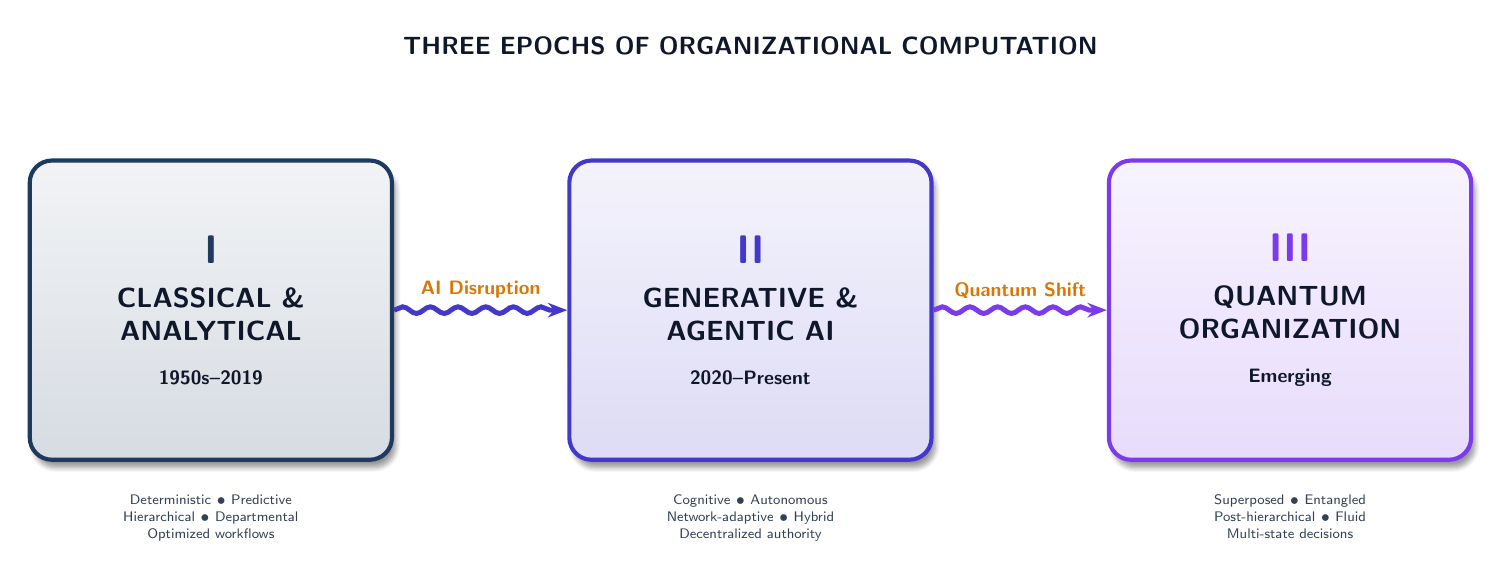
\begin{tikzpicture}[
  every node/.style={font=\sffamily},
  epoch/.style={
    rectangle, rounded corners=8pt,
    minimum width=4.6cm, minimum height=3.8cm,
    draw=#1, line width=1.5pt,
    top color=#1!6, bottom color=#1!18,
    font=\sffamily\bfseries,
    text=epochDark, align=center,
    blur shadow={shadow blur steps=6, shadow xshift=0.5mm, shadow yshift=-1mm}
  },
  sublabel/.style={
    font=\sffamily\tiny, text=epochSlate, align=center
  },
  transarrow/.style={
    -{Stealth[length=7pt]}, line width=1.8pt, #1,
    decorate, decoration={snake, amplitude=1.2pt, segment length=10pt, post length=5pt}
  },
]

% === EPOCH BOXES ===
\node[epoch=epochBlue] (e1) at (0,0) {
  {\Large\textcolor{epochBlue}{I}}\\[4pt]
  CLASSICAL \&\\ANALYTICAL\\[4pt]
  {\scriptsize 1950s--2019}
};

\node[epoch=epochIndigo, right=2.2cm of e1] (e2) {
  {\Large\textcolor{epochIndigo}{II}}\\[4pt]
  GENERATIVE \&\\AGENTIC AI\\[4pt]
  {\scriptsize 2020--Present}
};

\node[epoch=epochViolet, right=2.2cm of e2] (e3) {
  {\Large\textcolor{epochViolet}{III}}\\[4pt]
  QUANTUM\\ORGANIZATION\\[4pt]
  {\scriptsize Emerging}
};

% === Descriptors below ===
\node[sublabel, below=3mm of e1] {
  Deterministic $\bullet$ Predictive\\
  Hierarchical $\bullet$ Departmental\\
  Optimized workflows
};

\node[sublabel, below=3mm of e2] {
  Cognitive $\bullet$ Autonomous\\
  Network-adaptive $\bullet$ Hybrid\\
  Decentralized authority
};

\node[sublabel, below=3mm of e3] {
  Superposed $\bullet$ Entangled\\
  Post-hierarchical $\bullet$ Fluid\\
  Multi-state decisions
};

% === Transition Arrows ===
\draw[transarrow=epochIndigo]
  (e1.east) -- node[above, font=\sffamily\scriptsize\bfseries, text=epochAmber] {AI Disruption} (e2.west);
\draw[transarrow=epochViolet]
  (e2.east) -- node[above, font=\sffamily\scriptsize\bfseries, text=epochAmber] {Quantum Shift} (e3.west);

% === Top Label ===
\node[font=\sffamily\small\bfseries, text=epochDark, above=12mm of e2] {
  THREE EPOCHS OF ORGANIZATIONAL COMPUTATION
};

\end{tikzpicture}%
}
\caption{\textbf{The Three Epochs of Organizational Computation.} Each computing paradigm enables and constrains a distinct class of organizational forms. Transitions are not smooth adoptions but structural disruptions that reshape authority, governance, and coordination.}
\label{fig:three-epochs}
\end{figure*}


% ============================================================================
\section{Epoch I: The Classical Organization}
\label{sec:epoch-classical}

The modern corporation is, in a very real sense, a product of classical computing. The organizational structures we take for granted---hierarchies, departments, matrix organizations, ERP-driven processes---were shaped by the capabilities and constraints of deterministic, sequential computation.

\subsection{The Spreadsheet Shaped the Manager}

VisiCalc (1979) and Lotus 1-2-3 (1983) did not merely give managers a new tool---they reshaped what management \textit{was}. The spreadsheet imposed a worldview: reality is tabular, relationships are formulaic, and outcomes are deterministic functions of inputs.

This computational metaphor became the managerial metaphor:
\begin{itemize}[leftmargin=1.5em]
  \item \textbf{Budgets as spreadsheets} --- Financial planning became cell-by-cell allocation, reinforcing departmental silos.
  \item \textbf{Forecasts as extrapolation} --- The spreadsheet's ``drag to fill'' became the dominant planning paradigm: the future is a linear extension of the past.
  \item \textbf{Performance as metrics} --- What could be put in a cell became what was measured; what could not be quantified was invisible.
\end{itemize}

The spreadsheet did not just serve the hierarchy---it \textit{justified} it. Each management layer existed to aggregate, transform, and relay tabular information upward and decompose directives downward.

\subsection{The Database Shaped the Enterprise}

The relational database (Codd, 1970) provided the computational substrate for the enterprise. Its organizing principles---normalized tables, foreign keys, ACID transactions---mapped directly onto organizational principles:

\begin{table}[H]
\centering
\small
\begin{tabular}{@{} >{\raggedright\arraybackslash}p{3.2cm} >{\raggedright\arraybackslash}p{4.2cm} @{}}
\toprule
\textbf{Database Concept} & \textbf{Organizational Analog} \\
\midrule
Normalized tables    & Functional departments \\[6pt]
Foreign keys         & Cross-departmental references \\[6pt]
ACID transactions    & Approval workflows \\[6pt]
Schema constraints   & Policy \& compliance rules \\[6pt]
Backup \& recovery   & Audit trails \& archives \\
\bottomrule
\end{tabular}
\caption{Relational Database $\leftrightarrow$ Organizational Structure}
\label{tab:db-org-mapping}
\end{table}

ERP systems (SAP R/3, Oracle Applications) made this mapping explicit: the enterprise \textit{was} its database schema. Organizational change required schema migration. Business processes were transaction sequences. The corporation became a relational database with a legal entity attached.

\subsection{The Network Shaped the Supply Chain}

TCP/IP and the internet did not create globalization, but they made it computationally \textit{feasible}. B2B integration, EDI, and web services enabled supply chains that spanned continents---but only in the forms that packet-switched, request-response networking could support: sequential, handshake-based, and fundamentally synchronous in design even when asynchronous in implementation.

\subsection{Classical Constraints on Organization}

The classical computing paradigm imposed specific constraints on organizational form:

\begin{enumerate}[leftmargin=1.5em]
  \item \textbf{Sequential decision-making}: Decisions were processed one at a time through approval chains, because the underlying computation was sequential.
  \item \textbf{Hierarchical information flow}: Information moved up and down defined channels, because databases enforced schema and access control.
  \item \textbf{Deterministic planning}: Strategy was plan-then-execute, because computation was deterministic---given the same inputs, you expected the same outputs.
  \item \textbf{Bounded coordination}: The number of entities that could be coordinated was limited by computational throughput, favoring large, vertically integrated firms.
\end{enumerate}

These were not \textit{choices}---they were \textit{constraints}. Organizations were hierarchical because the computation available to them was sequential. They could not be otherwise.

\subsection{The 2010s: The Limits of Analytical ML}

Before the emergence of generative models, the deep learning boom of the 2010s introduced predictive analytics, recommendation engines, and pattern recognition at scale. However, this first wave of artificial intelligence did not restructure the human organization. Instead, it served as an advanced predictive input into the existing classical paradigm. 

Forecasts became more accurate and targeting became more precise, but decisions were still routed through sequential, hierarchical approval chains, and departments remained siloed. The computational capacity was used to optimize classical structures, not to transform them. The true disruption of authority and organizational form awaited the cognitive fluency and agentic capabilities of the next epoch.


% ============================================================================
\section{Epoch II: The Generative \& Agentic Organization}
\label{sec:epoch-ai}

The transition from classical and analytical frameworks to the generative and agentic organization is the defining structural disruption of the 2020s. While the previous decade used predictive models to optimize existing structures, the current epoch uses cognitive, autonomous models to fundamentally restructure authority and collapse traditional information relay layers.

\subsection{AI as Authority Restructuring}

The conventional narrative frames AI as a tool that automates tasks. This dramatically understates the organizational impact. AI does not merely perform tasks faster---it \textbf{redistributes the cognitive work} that justified organizational structure.

Consider the role of middle management. In the classical organization, middle managers exist primarily as \textit{information processors}:
\begin{itemize}[leftmargin=1.5em]
  \item \textbf{Upward}: Aggregating operational data into reports for senior leadership.
  \item \textbf{Downward}: Translating strategic directives into operational instructions.
  \item \textbf{Lateral}: Coordinating across departments that share no direct data links.
\end{itemize}

AI systems---large language models, analytics engines, decision-support platforms---now perform all three functions faster, with broader context, and with fewer distortions. The organizational implication is structural:

\begin{quote}
\textit{The hierarchy flattens not because of management ideology, but because the computational justification for information relay layers disappears.}
\end{quote}

This does not mean middle management is eliminated. It means middle management is \textit{transformed}: from information relay to \textbf{model governance}, \textbf{AI-human interface design}, and \textbf{ethical oversight}---roles that require judgment, not data aggregation.


% ============================================================================
% DIAGRAM 2: Classical vs. Generative & Agentic Authority Structure
% ============================================================================
\begin{figure*}[t]
\centering
\resizebox{0.92\textwidth}{!}{%
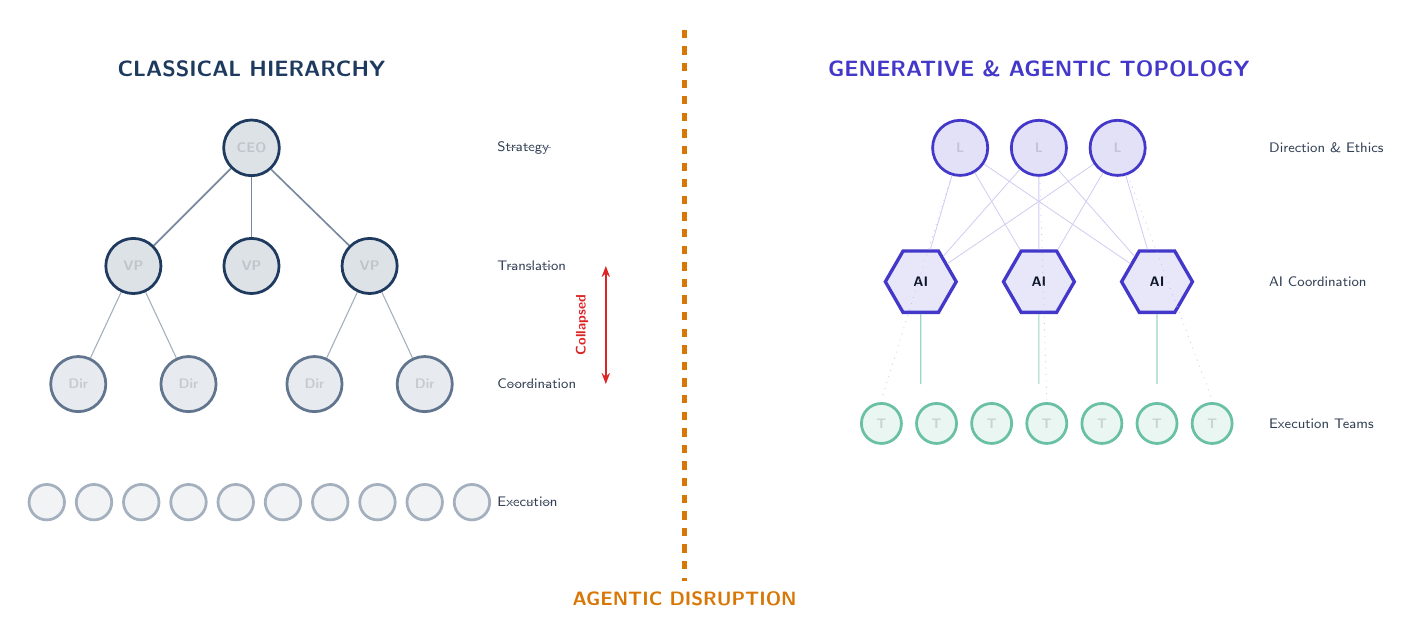
\begin{tikzpicture}[
  every node/.style={font=\sffamily\small},
  person/.style={
    circle, minimum size=0.7cm,
    draw=#1, line width=1pt,
    fill=#1, fill opacity=0.15, text=epochDark,
    font=\sffamily\tiny\bfseries
  },
  ainode/.style={
    regular polygon, regular polygon sides=6,
    minimum size=0.9cm,
    draw=epochIndigo, line width=1.2pt,
    fill=epochIndigo!12, text=epochDark,
    font=\sffamily\tiny\bfseries
  },
  grouplabel/.style={
    font=\sffamily\footnotesize\bfseries, text=#1
  },
]

% === CLASSICAL SIDE ===
\node[grouplabel=epochBlue] at (-5,4.5) {CLASSICAL HIERARCHY};

% CEO
\node[person=epochBlue] (c-ceo) at (-5,3.5) {CEO};
% VPs
\node[person=epochBlue] (c-vp1) at (-6.5,2) {VP};
\node[person=epochBlue] (c-vp2) at (-5,2) {VP};
\node[person=epochBlue] (c-vp3) at (-3.5,2) {VP};
% Directors
\node[person=epochBlue!70] (c-d1) at (-7.2,0.5) {Dir};
\node[person=epochBlue!70] (c-d2) at (-5.8,0.5) {Dir};
\node[person=epochBlue!70] (c-d3) at (-4.2,0.5) {Dir};
\node[person=epochBlue!70] (c-d4) at (-2.8,0.5) {Dir};
% Managers
\foreach \x in {-7.6,-7,-6.4,-5.8,-5.2,-4.6,-4,-3.4,-2.8,-2.2} {
  \node[person=epochBlue!40, minimum size=0.45cm] at (\x,-1) {};
}

% Classical connections
\draw[epochBlue!60, line width=0.6pt] (c-ceo) -- (c-vp1);
\draw[epochBlue!60, line width=0.6pt] (c-ceo) -- (c-vp2);
\draw[epochBlue!60, line width=0.6pt] (c-ceo) -- (c-vp3);
\draw[epochBlue!40, line width=0.4pt] (c-vp1) -- (c-d1);
\draw[epochBlue!40, line width=0.4pt] (c-vp1) -- (c-d2);
\draw[epochBlue!40, line width=0.4pt] (c-vp3) -- (c-d3);
\draw[epochBlue!40, line width=0.4pt] (c-vp3) -- (c-d4);

% Labels
\node[font=\sffamily\tiny, text=epochSlate, right] at (-2,3.5) {Strategy};
\node[font=\sffamily\tiny, text=epochSlate, right] at (-2,2) {Translation};
\node[font=\sffamily\tiny, text=epochSlate, right] at (-2,0.5) {Coordination};
\node[font=\sffamily\tiny, text=epochSlate, right] at (-2,-1) {Execution};

% Arrow labels
\draw[epochSlate!50, line width=0.3pt, dashed] (-1.2,3.5) -- (-1.8,3.5);
\draw[epochSlate!50, line width=0.3pt, dashed] (-1.2,2) -- (-1.8,2);
\draw[epochSlate!50, line width=0.3pt, dashed] (-1.2,0.5) -- (-1.8,0.5);
\draw[epochSlate!50, line width=0.3pt, dashed] (-1.2,-1) -- (-1.8,-1);

% === SEPARATOR ===
\draw[epochAmber, line width=1.5pt, dashed] (0.5,5) -- (0.5,-2)
  node[below, font=\sffamily\scriptsize\bfseries, text=epochAmber] {AGENTIC DISRUPTION};

% === GENERATIVE & AGENTIC SIDE ===
\node[grouplabel=epochIndigo] at (5,4.5) {GENERATIVE \& AGENTIC TOPOLOGY};

% Leadership (smaller layer)
\node[person=epochIndigo] (a-l1) at (4,3.5) {L};
\node[person=epochIndigo] (a-l2) at (5,3.5) {L};
\node[person=epochIndigo] (a-l3) at (6,3.5) {L};

% AI Layer (center)
\node[ainode] (ai1) at (3.5,1.8) {AI};
\node[ainode] (ai2) at (5,1.8) {AI};
\node[ainode] (ai3) at (6.5,1.8) {AI};

% Teams (direct connection)
\foreach \x in {3,3.7,4.4,5.1,5.8,6.5,7.2} {
  \node[person=epochGreen!60, minimum size=0.5cm] at (\x,0) {T};
}

% Generative/agentic connections (network, not tree)
\foreach \l in {a-l1, a-l2, a-l3} {
  \foreach \a in {ai1, ai2, ai3} {
    \draw[epochIndigo!25, line width=0.3pt] (\l) -- (\a);
  }
}

% AI to teams
\draw[epochGreen!40, line width=0.4pt] (ai1) -- ++(0,-1.3);
\draw[epochGreen!40, line width=0.4pt] (ai2) -- ++(0,-1.3);
\draw[epochGreen!40, line width=0.4pt] (ai3) -- ++(0,-1.3);

% Direct leader-team connections (bypassing layers)
\draw[epochIndigo!30, line width=0.3pt, dotted] (a-l1) -- (3,0.3);
\draw[epochIndigo!30, line width=0.3pt, dotted] (a-l2) -- (5.1,0.3);
\draw[epochIndigo!30, line width=0.3pt, dotted] (a-l3) -- (7.2,0.3);

% Right labels
\node[font=\sffamily\tiny, text=epochSlate, right] at (7.8,3.5) {Direction \& Ethics};
\node[font=\sffamily\tiny, text=epochSlate, right] at (7.8,1.8) {AI Coordination};
\node[font=\sffamily\tiny, text=epochSlate, right] at (7.8,0) {Execution Teams};

% Collapsed layers annotation
\draw[epochRed, line width=0.8pt, {Stealth[length=4pt]}-{Stealth[length=4pt]}]
  (-0.5,2) -- (-0.5,0.5);
\node[font=\sffamily\tiny\bfseries, text=epochRed, rotate=90] at (-0.8,1.25) {Collapsed};

\end{tikzpicture}%
}
\caption{\textbf{Authority Structure: Classical vs. Generative \& Agentic.} Left: The classical hierarchy with four layers (strategy, translation, coordination, execution). Right: The generative \& agentic topology where cognitive systems absorb the translation and coordination layers, creating direct connections between leadership (direction \& ethics) and execution teams. The middle layers are transformed into governance and oversight roles.}
\label{fig:classical-vs-ai}
\end{figure*}


\subsection{Five Emerging Human-AI Topologies}

As AI absorbs information relay functions, new organizational archetypes are emerging. We identify five, ordered by the degree of human-AI integration:

\subsubsection{The Centaur Model}
Named after the ``centaur chess'' phenomenon where human-AI pairs outperformed both humans and AI alone, the Centaur Model places a human-AI pair at every significant decision point. The human provides judgment, ethics, and contextual awareness; the AI provides data processing, pattern recognition, and option generation.

\textbf{Organizational signature}: Every role has an AI counterpart. Decision quality improves, but organizational speed is bounded by human deliberation.

\subsubsection{The Swarm Model}
Large fleets of AI agents---each specialized for narrow tasks---are coordinated by a small human leadership layer that sets objectives and constraints. Execution is fully autonomous within defined boundaries.

\textbf{Organizational signature}: Very high throughput, very flat structure, but governance complexity increases exponentially with the number of autonomous agents.

\subsubsection{The Conductor Model}
Humans function as orchestra conductors: they do not play instruments, but they shape tempo, dynamics, and interpretation. AI ensembles execute operational work while humans set strategic direction and intervene only when the performance deviates from intent.

\textbf{Organizational signature}: High scalability, clear separation of human and AI responsibilities, but risk of ``conductor's illusion''---believing you control what you merely observe.

\subsubsection{The Avatar Model}
The inverse of the Conductor, the Avatar Model places the AI system at the center of planning, orchestration, and scheduling, while humans serve as physical or localized execution units (the ``avatars''). This model is already present in early forms like ``algorithmic management'' in the gig economy (e.g., routing drivers or scheduling logistics). In its advanced form, AI models determine real-time task allocations and operational goals, and dispatch human agents to execute high-dexterity, creative, or empathetic tasks that cannot be performed digitally.

\textbf{Organizational signature}: High operational efficiency and task optimization, but risk of dehumanization, erosion of worker agency, and extreme commoditization of human labor.

\subsubsection{The Symbiote Model}
Deep integration where human cognition and AI analysis become inseparable at the individual and team level. The organization does not assign tasks to ``humans'' or ``AI''---it assigns tasks to \textit{hybrid cognitive units} that think as integrated entities.

\textbf{Organizational signature}: Maximum adaptability, but raises profound questions about identity, agency, and accountability.


% ============================================================================
% DIAGRAM 3: Five Human-AI Organizational Topologies
% ============================================================================
\begin{figure*}[t]
\centering
\resizebox{\textwidth}{!}{%
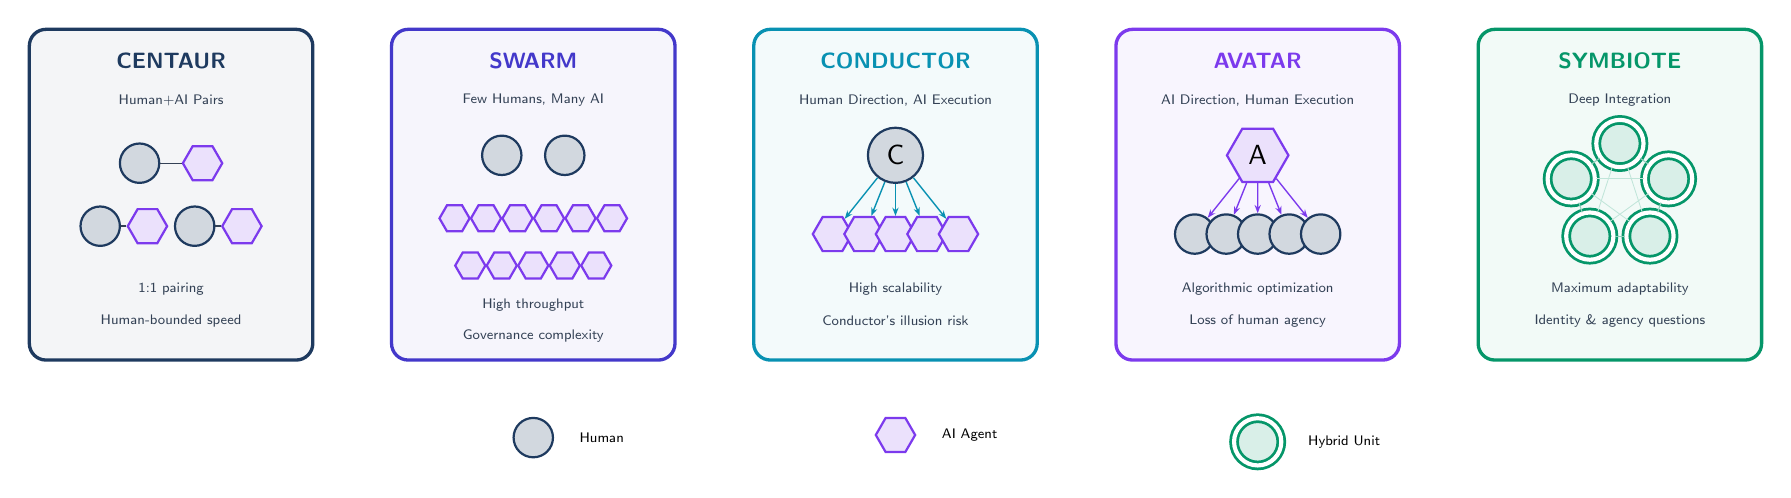
\begin{tikzpicture}[
  every node/.style={font=\sffamily},
  modelbox/.style={
    rectangle, rounded corners=6pt,
    minimum width=3.6cm, minimum height=4.2cm,
    draw=#1, line width=1.2pt,
    fill=#1!5, text=epochDark, align=center
  },
  human/.style={
    circle, minimum size=0.5cm,
    draw=epochBlue, line width=0.8pt,
    fill=epochBlue!20
  },
  ai/.style={
    regular polygon, regular polygon sides=6,
    minimum size=0.5cm,
    draw=epochViolet, line width=0.8pt,
    fill=epochViolet!15
  },
  hybrid/.style={
    circle, minimum size=0.6cm,
    draw=epochGreen, line width=1pt,
    fill=epochGreen!15,
    double, double distance=1.5pt
  },
]

% === CENTAUR ===
\node[modelbox=epochBlue] (m1) at (0,0) {};
\node[font=\sffamily\footnotesize\bfseries, text=epochBlue] at (0,1.7) {CENTAUR};
\node[font=\sffamily\tiny, text=epochSlate] at (0,1.2) {Human+AI Pairs};

% Centaur pairs (properly separated and aligned)
\node[human] (c-h1) at (-0.4,0.4) {};
\node[ai] (c-a1) at (0.4,0.4) {};
\draw[epochSlate, line width=0.5pt] (c-h1) -- (c-a1);

\node[human] (c-h2) at (-0.9,-0.4) {};
\node[ai] (c-a2) at (-0.3,-0.4) {};
\draw[epochSlate, line width=0.5pt] (c-h2) -- (c-a2);

\node[human] (c-h3) at (0.3,-0.4) {};
\node[ai] (c-a3) at (0.9,-0.4) {};
\draw[epochSlate, line width=0.5pt] (c-h3) -- (c-a3);

\node[font=\sffamily\tiny, text=epochSlate] at (0,-1.2) {1:1 pairing};
\node[font=\sffamily\tiny, text=epochSlate] at (0,-1.6) {Human-bounded speed};

% === SWARM ===
\node[modelbox=epochIndigo] (m2) at (4.6,0) {};
\node[font=\sffamily\footnotesize\bfseries, text=epochIndigo] at (4.6,1.7) {SWARM};
\node[font=\sffamily\tiny, text=epochSlate] at (4.6,1.2) {Few Humans, Many AI};

% Few humans at top
\node[human] (s-h1) at (4.2,0.5) {};
\node[human] (s-h2) at (5.0,0.5) {};

% Many AI below
\foreach \x in {3.6,4.0,4.4,4.8,5.2,5.6} {
  \node[ai, minimum size=0.35cm] at (\x,-0.3) {};
}
\foreach \x in {3.8,4.2,4.6,5.0,5.4} {
  \node[ai, minimum size=0.35cm] at (\x,-0.9) {};
}

\node[font=\sffamily\tiny, text=epochSlate] at (4.6,-1.4) {High throughput};
\node[font=\sffamily\tiny, text=epochSlate] at (4.6,-1.8) {Governance complexity};

% === CONDUCTOR ===
\node[modelbox=epochCyan] (m3) at (9.2,0) {};
\node[font=\sffamily\footnotesize\bfseries, text=epochCyan] at (9.2,1.7) {CONDUCTOR};
\node[font=\sffamily\tiny, text=epochSlate] at (9.2,1.2) {Human Direction, AI Execution};

% Conductor (human) at top
\node[human, minimum size=0.7cm] (cond) at (9.2,0.5) {C};

% AI ensemble below
\node[ai] (ai1) at (8.4,-0.5) {};
\node[ai] (ai2) at (8.8,-0.5) {};
\node[ai] (ai3) at (9.2,-0.5) {};
\node[ai] (ai4) at (9.6,-0.5) {};
\node[ai] (ai5) at (10.0,-0.5) {};

% Direction arrows (fan configuration to all agents)
\foreach \i in {1,2,3,4,5} {
  \draw[epochCyan, line width=0.5pt, -{Stealth[length=3pt]}] (cond) -- (ai\i);
}

\node[font=\sffamily\tiny, text=epochSlate] at (9.2,-1.2) {High scalability};
\node[font=\sffamily\tiny, text=epochSlate] at (9.2,-1.6) {Conductor's illusion risk};

% === AVATAR ===
\node[modelbox=epochViolet] (m4) at (13.8,0) {};
\node[font=\sffamily\footnotesize\bfseries, text=epochViolet] at (13.8,1.7) {AVATAR};
\node[font=\sffamily\tiny, text=epochSlate] at (13.8,1.2) {AI Direction, Human Execution};

% AI conductor at top
\node[ai, minimum size=0.7cm] (avatar-ai) at (13.8,0.5) {A};

% Human executors below
\node[human] (h1) at (13.0,-0.5) {};
\node[human] (h2) at (13.4,-0.5) {};
\node[human] (h3) at (13.8,-0.5) {};
\node[human] (h4) at (14.2,-0.5) {};
\node[human] (h5) at (14.6,-0.5) {};

% Direction arrows (fan configuration from AI to humans)
\foreach \i in {1,2,3,4,5} {
  \draw[epochViolet, line width=0.5pt, -{Stealth[length=3pt]}] (avatar-ai) -- (h\i);
}

\node[font=\sffamily\tiny, text=epochSlate] at (13.8,-1.2) {Algorithmic optimization};
\node[font=\sffamily\tiny, text=epochSlate] at (13.8,-1.6) {Loss of human agency};

% === SYMBIOTE ===
\node[modelbox=epochGreen] (m5) at (18.4,0) {};
\node[font=\sffamily\footnotesize\bfseries, text=epochGreen] at (18.4,1.7) {SYMBIOTE};
\node[font=\sffamily\tiny, text=epochSlate] at (18.4,1.2) {Deep Integration};

% Hybrid nodes (calculated placement on a clean circle to prevent overlap)
\node[hybrid] (s1) at ($(18.4,0) + (162:0.65cm)$) {};
\node[hybrid] (s2) at ($(18.4,0) + (90:0.65cm)$) {};
\node[hybrid] (s3) at ($(18.4,0) + (18:0.65cm)$) {};
\node[hybrid] (s4) at ($(18.4,0) + (306:0.65cm)$) {};
\node[hybrid] (s5) at ($(18.4,0) + (234:0.65cm)$) {};

% Fully connected network mesh (connected to boundaries, not centers)
\draw[epochGreen!45, line width=0.4pt] (s1) -- (s2);
\draw[epochGreen!45, line width=0.4pt] (s2) -- (s3);
\draw[epochGreen!45, line width=0.4pt] (s3) -- (s4);
\draw[epochGreen!45, line width=0.4pt] (s4) -- (s5);
\draw[epochGreen!45, line width=0.4pt] (s5) -- (s1);

\draw[epochGreen!25, line width=0.3pt] (s1) -- (s3);
\draw[epochGreen!25, line width=0.3pt] (s1) -- (s4);
\draw[epochGreen!25, line width=0.3pt] (s2) -- (s4);
\draw[epochGreen!25, line width=0.3pt] (s2) -- (s5);
\draw[epochGreen!25, line width=0.3pt] (s3) -- (s5);

\node[font=\sffamily\tiny, text=epochSlate] at (18.4,-1.2) {Maximum adaptability};
\node[font=\sffamily\tiny, text=epochSlate] at (18.4,-1.6) {Identity \& agency questions};

% === LEGEND ===
\node[human, below=0.7cm of m2] (leg-h) {};
\node[font=\sffamily\tiny, right=2mm of leg-h] {Human};
\node[ai, below=0.7cm of m3] (leg-a) {};
\node[font=\sffamily\tiny, right=2mm of leg-a] {AI Agent};
\node[hybrid, below=0.7cm of m4] (leg-hy) {};
\node[font=\sffamily\tiny, right=2mm of leg-hy] {Hybrid Unit};

\end{tikzpicture}%
}
\caption{\textbf{Five Human-AI Organizational Topologies.} Each model represents a different balance of human and AI roles. Centaur pairs humans with AI 1:1. Swarm deploys many AI agents under few human leaders. Conductor separates direction (human) from execution (AI). Avatar features AI-driven orchestration with human execution. Symbiote fuses human and AI into indivisible hybrid cognitive units.}
\label{fig:five-topologies}
\end{figure*}


\subsection{The Three Pressures of AI Transition}

Organizations in Epoch II face three simultaneous structural pressures:

\subsubsection{Compression of Decision Latency}
AI collapses the time between sensing a condition and acting on it. Classical organizations processed decisions through layers---each layer adding latency but also adding judgment. AI removes the latency while claiming to preserve (or improve) the judgment.

The organizational consequence: \textbf{layers that existed to add judgment must now prove they add judgment that AI cannot.} If a layer exists only to relay and aggregate, it is computationally redundant.

\subsubsection{Expansion of Decision Dimensionality}
AI handles more variables simultaneously than any human or team of humans. A pricing decision that once considered five factors (cost, competition, demand, margin target, and inventory) now considers five hundred (adding weather, social sentiment, competitor real-time pricing, individual customer history, geopolitical risk, and so on).

The organizational consequence: \textbf{decision authority migrates from ``the person who understands the domain'' to ``the system that can process the most dimensions.''} Human authority becomes oversight authority---ensuring the system's objectives are aligned, not performing the computation itself.

\subsubsection{Dissolution of Departmental Boundaries}
When AI systems process data across the entire organization simultaneously, the departmental boundaries that existed to partition computational load become artificial. A customer service AI that can access supply chain data, financial records, and product engineering specifications in real-time dissolves the boundaries between four departments in a single query.

The organizational consequence: \textbf{functional departments persist as centers of expertise, but cease to function as information boundaries.} The ``wall'' between sales and operations becomes a ``membrane'' through which AI flows freely.


\subsection{Governance in the Generative \& Agentic Organization}

The governance challenges of Epoch II are qualitatively different from Epoch I:

\begin{table}[H]
\centering
\small
\begin{tabular}{@{} >{\raggedright\arraybackslash}p{2.6cm} >{\raggedright\arraybackslash}p{4.8cm} @{}}
\toprule
\textbf{Challenge} & \textbf{Description} \\
\midrule
Accountability gap & When AI makes a harmful decision, who is responsible? The designer? The operator? The organization? \\[6pt]
Explainability--speed tradeoff & Faster AI decisions are harder to explain. Organizations must choose their position on this spectrum. \\[6pt]
Skill displacement & Roles defined by information processing are automated, creating workforce dislocation. \\[6pt]
AI agent legal status & If an AI agent negotiates a contract, what are the legal implications? \\[6pt]
Audit velocity & Decisions made in milliseconds cannot be audited at human speed. \\
\bottomrule
\end{tabular}
\caption{Governance Challenges in the Generative \& Agentic Organization}
\label{tab:ai-governance}
\end{table}


% ============================================================================
\section{Epoch III: The Quantum Organization}
\label{sec:epoch-quantum}

If Epoch II restructures the organization by compressing information processing, Epoch III restructures the organization by \textit{expanding the space of possible computations}. Quantum computing does not just make existing computations faster---it makes \textbf{previously impossible computations possible}. And if organizational form is constrained by computational capacity, then quantum computing enables organizational forms that are currently inconceivable.

\subsection{What Quantum Computing Actually Changes}

Grounded in Feynman's original insight, quantum computing enables four categories of capability that are qualitatively different from classical or AI computation:

\begin{enumerate}[leftmargin=1.5em]
  \item \textbf{Combinatorial optimization at scale}: Problems with exponentially many possible solutions---portfolio optimization, logistics routing, resource allocation across millions of variables---can be explored simultaneously through quantum superposition, rather than sequentially.
  \item \textbf{True simulation of complex systems}: Molecular interactions, market dynamics, organizational behavior, and social network effects can be modeled at a fidelity impossible for classical computers, because the simulation medium matches the phenomenon's quantum nature.
  \item \textbf{Cryptographic paradigm shift}: Shor's algorithm \cite{shor1994} threatens current public-key cryptography, forcing a complete rethink of digital trust, identity, and contract enforcement---the computational substrate of governance.
  \item \textbf{Quantum machine learning}: Access to feature spaces and pattern structures that classical ML cannot represent, enabling recognition of organizational patterns invisible to classical analysis.
\end{enumerate}

\subsection{The Entangled Organization --- A Conceptual Framework}

We introduce the concept of the \textbf{Entangled Organization}---an organizational form that borrows structural principles from quantum mechanics, not as metaphor alone, but as descriptions of computationally-enabled coordination patterns.

\subsubsection{Decision Entanglement}
In classical organizations, strategy and operations are sequential: strategy is formulated, then executed. In generative and agentic organizations, feedback loops tighten this sequence. In the quantum organization, strategy and operations are \textit{entangled}---changes in operational reality \textit{instantaneously} reshape strategy, and strategic shifts \textit{instantaneously} reconfigure operations.

This is not real-time feedback (which is still classical---sense, process, respond). It is \textit{structural coupling}: strategy and operations exist as a single quantum state that cannot be decomposed into independent components.

\subsubsection{Resource Superposition}
In classical organizations, resources are allocated: a dollar is in one budget, a person is on one team. In the entangled organization, resources exist in \textit{superposition} across multiple potential uses until a decision \textit{collapses} them into a specific allocation.

This is computationally meaningful: quantum optimization can maintain all possible resource configurations simultaneously and collapse to the optimal one when a commitment is required, rather than pre-allocating resources based on forecasts.

\subsubsection{The Organizational Measurement Problem}
In quantum mechanics, observation collapses a superposed state into a definite one. In organizations, \textit{measurement}---reporting, KPIs, audits---may similarly \textit{alter} the system being measured. A team that is ``measured'' on velocity may optimize for velocity at the expense of quality, not because of incentive misalignment, but because measurement itself collapses the superposition of possible behaviors into the measured one.

Quantum-aware organizations must design for this: measurement strategies that extract information without collapsing the adaptive potential of the system.


% ============================================================================
% DIAGRAM 4: The Entangled Organization
% ============================================================================
\begin{figure*}[t]
\centering
\resizebox{0.75\textwidth}{!}{%
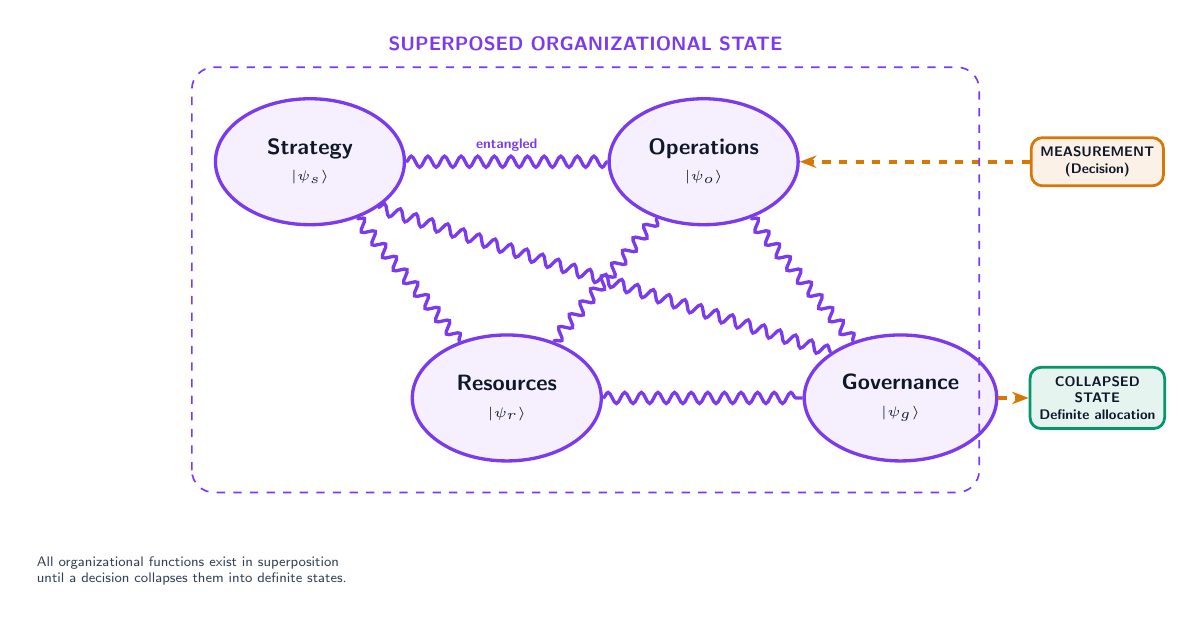
\begin{tikzpicture}[
  every node/.style={font=\sffamily},
  qstate/.style={
    ellipse, minimum width=2.4cm, minimum height=1.6cm,
    draw=epochViolet, line width=1.2pt,
    fill=epochViolet!8, text=epochDark,
    font=\sffamily\footnotesize\bfseries, align=center
  },
  entangle/.style={
    epochViolet, line width=1.2pt,
    decorate, decoration={snake, amplitude=2pt, segment length=6pt}
  },
  collapse/.style={
    -{Stealth[length=6pt]}, epochAmber, line width=1.5pt, dashed
  },
]

% Quantum states
\node[qstate] (strat) at (0,3) {Strategy\\{\tiny$|\psi_s\rangle$}};
\node[qstate] (ops) at (5,3) {Operations\\{\tiny$|\psi_o\rangle$}};
\node[qstate] (res) at (2.5,0) {Resources\\{\tiny$|\psi_r\rangle$}};
\node[qstate] (gov) at (7.5,0) {Governance\\{\tiny$|\psi_g\rangle$}};

% Entanglement connections
\draw[entangle] (strat) -- node[above, font=\sffamily\tiny\bfseries, text=epochViolet] {entangled} (ops);
\draw[entangle] (strat) -- (res);
\draw[entangle] (ops) -- (res);
\draw[entangle] (ops) -- (gov);
\draw[entangle] (res) -- (gov);
\draw[entangle] (strat.south east) -- (gov.north west);

% Measurement/collapse
\node[rectangle, rounded corners=4pt, draw=epochAmber, line width=1pt, fill=epochAmber!10,
  font=\sffamily\tiny\bfseries, text=epochDark, align=center] (meas) at (10,3) {
  MEASUREMENT\\(Decision)
};
\draw[collapse] (meas.west) -- (ops.east);

% Collapsed state
\node[rectangle, rounded corners=4pt, draw=epochGreen, line width=1pt, fill=epochGreen!10,
  font=\sffamily\tiny\bfseries, text=epochDark, align=center] (collapsed) at (10,0) {
  COLLAPSED\\STATE\\{\tiny Definite allocation}
};
\draw[collapse] (gov.east) -- (collapsed.west);

% Superposition label
\node[font=\sffamily\scriptsize\bfseries, text=epochViolet] at (3.5,4.5) {
  SUPERPOSED ORGANIZATIONAL STATE
};
\draw[epochViolet, line width=0.6pt, dashed, rounded corners=8pt]
  (-1.5,-1.2) rectangle (8.5,4.2);

% Annotations
\node[font=\sffamily\tiny, text=epochSlate, align=left] at (-1.5,-2.2) {
  All organizational functions exist in superposition\\
  until a decision collapses them into definite states.
};

\end{tikzpicture}%
}
\caption{\textbf{The Entangled Organization.} Strategy, operations, resources, and governance exist as entangled quantum states in superposition. A decision (measurement) collapses the entangled system into a definite state. Changes to any component instantaneously affect all others through entanglement.}
\label{fig:entangled-org}
\end{figure*}


\subsection{The Feynman Organization}

We coin the term \textbf{Feynman Organization} to describe the ultimate expression of the quantum organizational concept:

\begin{quote}
\textit{A Feynman Organization is an enterprise that does not model its environment, but simulates it at full fidelity---using quantum computation to maintain a living digital twin of the entire organization-environment system, exploring all possible states simultaneously and collapsing to optimal decisions in real-time.}
\end{quote}

Just as Feynman argued that simulating quantum physics requires a quantum computer, we argue that simulating the full complexity of a modern enterprise operating in a complex market requires computation that operates at the same level of complexity as the system itself.

The Feynman Organization does not plan and then execute. It exists simultaneously in all possible plans and collapses to the best one when action is required. This is not metaphor---it is a description of what quantum optimization actually does, applied to organizational decision-making.

\subsection{Quantum-Era Governance}

If Epoch II's governance challenge is speed (decisions faster than audits), Epoch III's governance challenge is \textbf{dimensionality} (decisions across more dimensions than human comprehension can encompass):

\begin{table}[H]
\centering
\small
\begin{tabular}{@{} >{\raggedright\arraybackslash}p{1.9cm} >{\raggedright\arraybackslash}p{2.3cm} >{\raggedright\arraybackslash}p{3.0cm} @{}}
\toprule
\textbf{Epoch I} & \textbf{Epoch II} & \textbf{Epoch III} \\
\midrule
Sequential audit trails & Real-time AI compliance monitoring & Quantum-verified immutable audit \\[6pt]
Rule-based HR policy & Agentic talent matching & Quantum-optimized workforce superposition \\[6pt]
\hspace{0pt}Deterministic finance & Predictive financial modeling & Probabilistic financial states \\[6pt]
\hspace{0pt}Jurisdictional legal & \hspace{0pt}Cross-jurisdictional AI monitoring & Quantum-secured smart contracts \\
\bottomrule
\end{tabular}
\caption{Governance Evolution Across Three Epochs}
\label{tab:governance-evolution}
\end{table}


% ============================================================================
\section{The Transition: Preparing Now for Quantum}
\label{sec:transition}

Quantum computing is not yet mature for enterprise deployment at scale. But the architectural decisions organizations make \textit{today}---in the AI era---will determine whether they can transition smoothly into the quantum era or face catastrophic restructuring.

\subsection{Architectural Decisions That Enable Quantum Readiness}

\begin{enumerate}[leftmargin=1.5em]
  \item \textbf{Design for probabilistic outcomes}: Organizations that insist on deterministic outputs from AI systems will struggle to adapt to quantum's inherently probabilistic nature. Begin designing decision processes that accept and reason over probability distributions, not point estimates.

  \item \textbf{Decompose into quantum-compatible problem structures}: Quantum computers excel at specific problem classes---optimization, simulation, sampling. Organizations that have already decomposed their core challenges into these forms will be ready to apply quantum advantage.

  \item \textbf{Post-quantum cryptographic migration}: Begin transitioning to post-quantum cryptographic standards now. The governance infrastructure built on current encryption will be vulnerable when quantum computers reach sufficient scale.

  \item \textbf{Cultivate quantum literacy}: Not everyone needs to understand quantum physics, but leaders need to understand what quantum computing \textit{can and cannot do}---to avoid both dismissal and hype.

  \item \textbf{Invest in hybrid classical-quantum architectures}: The near-term reality is hybrid computation---classical systems handling routine work, quantum systems tackling specific high-value optimization and simulation problems. Design systems that can offload appropriate workloads to quantum processors as they become available.
\end{enumerate}

\subsection{What Must Survive Across All Epochs}

Not everything changes. Certain organizational principles persist across all three epochs, because they are not computationally contingent:

\begin{itemize}[leftmargin=1.5em]
  \item \textbf{Human agency}: Regardless of computational power, the decision about \textit{what to optimize for}---what values, what goals, what constraints---remains irreducibly human.
  \item \textbf{Accountability}: The chain of responsibility may restructure, but the \textit{principle} that decisions have consequences and consequences have owners persists.
  \item \textbf{Trust}: Organizations are trust structures. Computing can verify, validate, and enforce---but trust between humans is a social phenomenon that no computing paradigm replaces.
  \item \textbf{Purpose}: An organization must know \textit{why} it exists. Computing can optimize the \textit{how}; it cannot supply the \textit{why}.
\end{itemize}


% ============================================================================
% DIAGRAM 5: Organizational Evolution Timeline
% ============================================================================
\begin{figure*}[t]
\centering
\resizebox{\textwidth}{!}{%
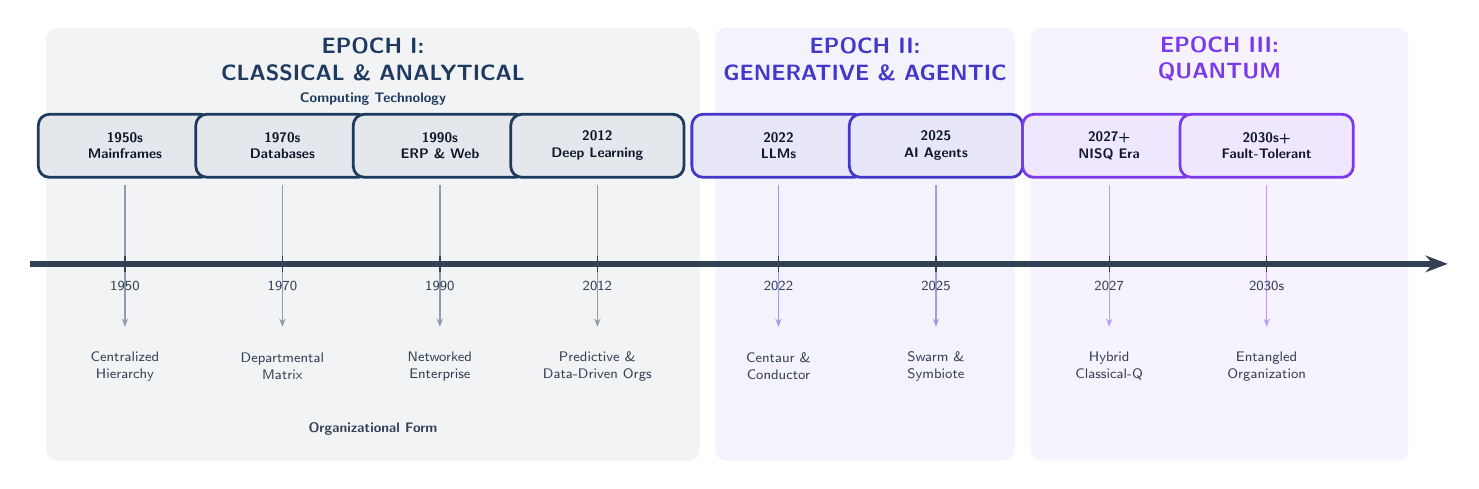
\begin{tikzpicture}[
  every node/.style={font=\sffamily},
  milestone/.style={
    rectangle, rounded corners=4pt,
    minimum width=2.2cm, minimum height=0.8cm,
    draw=#1, line width=1pt,
    fill=#1!12, text=epochDark,
    font=\sffamily\tiny\bfseries, align=center
  },
]

% Timeline axis
\draw[epochSlate, line width=2pt, -{Stealth[length=8pt]}]
  (0,0) -- (18,0);

% Era backgrounds
\begin{scope}[on background layer]
  \fill[epochBlue!6, rounded corners=4pt] (0.2,3) rectangle (8.5,-2.5);
  \fill[epochIndigo!6, rounded corners=4pt] (8.7,3) rectangle (12.5,-2.5);
  \fill[epochViolet!6, rounded corners=4pt] (12.7,3) rectangle (17.5,-2.5);
\end{scope}

% Era labels
\node[font=\sffamily\footnotesize\bfseries, text=epochBlue, align=center] at (4.35,2.6) {EPOCH I:\\CLASSICAL \& ANALYTICAL};
\node[font=\sffamily\footnotesize\bfseries, text=epochIndigo, align=center] at (10.6,2.6) {EPOCH II:\\GENERATIVE \& AGENTIC};
\node[font=\sffamily\footnotesize\bfseries, text=epochViolet, align=center] at (15.1,2.6) {EPOCH III:\\QUANTUM};

% Epoch I milestones
\node[milestone=epochBlue] at (1.2,1.5) {1950s\\Mainframes};
\node[milestone=epochBlue] at (3.2,1.5) {1970s\\Databases};
\node[milestone=epochBlue] at (5.2,1.5) {1990s\\ERP \& Web};
\node[milestone=epochBlue] at (7.2,1.5) {2012\\Deep Learning};

% Epoch I org forms
\node[font=\sffamily\tiny, text=epochSlate, align=center] at (1.2,-1.3) {Centralized\\Hierarchy};
\node[font=\sffamily\tiny, text=epochSlate, align=center] at (3.2,-1.3) {Departmental\\Matrix};
\node[font=\sffamily\tiny, text=epochSlate, align=center] at (5.2,-1.3) {Networked\\Enterprise};
\node[font=\sffamily\tiny, text=epochSlate, align=center] at (7.2,-1.3) {Predictive \&\\Data-Driven Orgs};

% Arrows down
\draw[epochBlue!50, line width=0.5pt, -{Stealth[length=3pt]}] (1.2,1.0) -- (1.2,-0.8);
\draw[epochBlue!50, line width=0.5pt, -{Stealth[length=3pt]}] (3.2,1.0) -- (3.2,-0.8);
\draw[epochBlue!50, line width=0.5pt, -{Stealth[length=3pt]}] (5.2,1.0) -- (5.2,-0.8);
\draw[epochBlue!50, line width=0.5pt, -{Stealth[length=3pt]}] (7.2,1.0) -- (7.2,-0.8);

% Epoch II milestones
\node[milestone=epochIndigo] at (9.5,1.5) {2022\\LLMs};
\node[milestone=epochIndigo] at (11.5,1.5) {2025\\AI Agents};

% Epoch II org forms
\node[font=\sffamily\tiny, text=epochSlate, align=center] at (9.5,-1.3) {Centaur \&\\Conductor};
\node[font=\sffamily\tiny, text=epochSlate, align=center] at (11.5,-1.3) {Swarm \&\\Symbiote};

\draw[epochIndigo!50, line width=0.5pt, -{Stealth[length=3pt]}] (9.5,1.0) -- (9.5,-0.8);
\draw[epochIndigo!50, line width=0.5pt, -{Stealth[length=3pt]}] (11.5,1.0) -- (11.5,-0.8);

% Epoch III milestones
\node[milestone=epochViolet] at (13.7,1.5) {2027+\\NISQ Era};
\node[milestone=epochViolet] at (15.7,1.5) {2030s+\\Fault-Tolerant};

% Epoch III org forms
\node[font=\sffamily\tiny, text=epochSlate, align=center] at (13.7,-1.3) {Hybrid\\Classical-Q};
\node[font=\sffamily\tiny, text=epochSlate, align=center] at (15.7,-1.3) {Entangled\\Organization};

\draw[epochViolet!50, line width=0.5pt, -{Stealth[length=3pt]}] (13.7,1.0) -- (13.7,-0.8);
\draw[epochViolet!50, line width=0.5pt, -{Stealth[length=3pt]}] (15.7,1.0) -- (15.7,-0.8);

% Year markers on timeline
\foreach \x/\yr in {1.2/1950, 3.2/1970, 5.2/1990, 7.2/2012, 9.5/2022, 11.5/2025, 13.7/2027, 15.7/2030s} {
  \draw[epochSlate, line width=0.5pt] (\x,-0.1) -- (\x,0.1);
  \node[font=\sffamily\tiny, text=epochSlate, below=1mm] at (\x,0) {\yr};
}

% Top labels
\node[font=\sffamily\tiny\bfseries, text=epochBlue] at (4.35,2.1) {Computing Technology};
\node[font=\sffamily\tiny\bfseries, text=epochSlate] at (4.35,-2.1) {Organizational Form};

\end{tikzpicture}%
}
\caption{\textbf{Organizational Evolution Timeline.} Computing milestones (top) and the organizational forms they enabled (bottom). Each computing paradigm shift triggers a structural organizational shift, with increasing speed of transition across epochs.}
\label{fig:timeline}
\end{figure*}


% ============================================================================
\section{Open Questions and Research Agenda}
\label{sec:questions}

This paper raises more questions than it answers---deliberately. The transition from generative and agentic to quantum organization is nascent, and premature prescription would be irresponsible. We close with the questions we believe are most urgent:

\subsection{Is Organizational Hierarchy an Artifact of Computational Limitation?}

If hierarchy exists because sequential computation required sequential information processing, and if quantum computation removes the sequential constraint, does hierarchy dissolve? Or does hierarchy serve functions---identity, belonging, clear authority---that are computationally irrelevant but socially essential?

\subsection{The Human Role in Quantum-Computed Enterprises}

If quantum simulation can model every possible outcome of every possible strategy simultaneously, does human judgment become irrelevant---or \textit{more} important as the selector of which outcomes to pursue? We argue the latter: quantum computing amplifies the importance of human values, because the system can optimize for \textit{any} objective, and choosing the right objective is irreducibly human.

\subsection{Governance Beyond Human Comprehension}

When decisions are made across more dimensions than human cognition can encompass, how does governance function? Classical governance assumes a human auditor can understand the decision being audited. AI governance assumes a human can understand the model's reasoning. Quantum governance may require accepting that some decisions are \textit{verified} without being \textit{understood}---a profound shift in the philosophy of accountability.

\subsection{Employment in the Quantum Enterprise}

If workforce allocation is itself a quantum optimization problem---finding the optimal assignment of people to roles across all possible configurations simultaneously---what does this mean for human agency, career development, and labor rights? Does the ``superposition of roles'' empower workers with flexibility or strip them of stable identity?

\subsection{Organizational Readiness Assessment}

How should organizations assess their readiness for the quantum transition? We propose that readiness is not a technology question but an \textit{architectural} one: can the organization accept probabilistic outcomes, decompose problems into quantum-compatible forms, and govern systems whose decision processes exceed human comprehension?


% ============================================================================
\section{Conclusion}
\label{sec:conclusion}

Feynman's insight was that nature demands to be simulated on its own terms. We extend this insight to organizations: \textit{organizations demand to be computed on the terms of the computing available to them}.

The classical computer gave us the hierarchical, departmental, plan-and-execute corporation. It was not a choice---it was a computational constraint. AI is now dissolving that constraint, flattening hierarchies, restructuring authority, and introducing hybrid human-AI organizational topologies that would have been impossible to coordinate with classical computation alone.

Quantum computing promises to dissolve constraints that even AI cannot touch: the constraint of sequential exploration, the constraint of deterministic resource allocation, the constraint of comprehensible-but-limited decision spaces. The organizations that emerge from the quantum era may be as different from today's generative and agentic enterprises as those enterprises are from the mainframe-era corporations of the 1960s.

The question for organizational leaders is not whether this transition will happen, but whether they will prepare for it---or be restructured by it.

\begin{quote}
\textit{``The question is not whether organizations will change in the age of AI and quantum computing. The question is whether organizations will change fast enough to remain coherent---or whether they will be dissolved and reformed by the forces they cannot outpace.''}
\end{quote}


{\small
\begin{thebibliography}{99}

\bibitem{feynman1982}
Feynman, R.P. (1982). ``Simulating Physics with Computers.'' \textit{International Journal of Theoretical Physics}, 21(6/7), 467--488.

\bibitem{simon1947}
Simon, H.A. (1947). \textit{Administrative Behavior: A Study of Decision-Making Processes in Administrative Organization}. Macmillan.

\bibitem{galbraith1974}
Galbraith, J.R. (1974). ``Organization Design: An Information Processing View.'' \textit{Interfaces}, 4(3), 28--36.

\bibitem{coase1937}
Coase, R.H. (1937). ``The Nature of the Firm.'' \textit{Economica}, 4(16), 386--405.

\bibitem{shor1994}
Shor, P.W. (1994). ``Algorithms for Quantum Computation: Discrete Logarithms and Factoring.'' \textit{Proceedings of the 35th Annual Symposium on Foundations of Computer Science}, 124--134.

\bibitem{preskill2018}
Preskill, J. (2018). ``Quantum Computing in the NISQ Era and Beyond.'' \textit{Quantum}, 2, 79.

\bibitem{brynjolfsson2014}
Brynjolfsson, E. \& McAfee, A. (2014). \textit{The Second Machine Age: Work, Progress, and Prosperity in a Time of Brilliant Technologies}. W.W. Norton.

\bibitem{laloux2014}
Laloux, F. (2014). \textit{Reinventing Organizations: A Guide to Creating Organizations Inspired by the Next Stage of Human Consciousness}. Nelson Parker.

\bibitem{zuboff2019}
Zuboff, S. (2019). \textit{The Age of Surveillance Capitalism: The Fight for a Human Future at the New Frontier of Power}. PublicAffairs.

\bibitem{nielsen2010}
Nielsen, M.A. \& Chuang, I.L. (2010). \textit{Quantum Computation and Quantum Information: 10th Anniversary Edition}. Cambridge University Press.

\bibitem{codd1970}
Codd, E.F. (1970). ``A Relational Model of Data for Large Shared Data Banks.'' \textit{Communications of the ACM}, 13(6), 377--387.

\bibitem{williamson1975}
Williamson, O.E. (1975). \textit{Markets and Hierarchies: Analysis and Antitrust Implications}. Free Press.

\end{thebibliography}}


\vspace{12pt}
\noindent\rule{\columnwidth}{0.3pt}
\vspace{6pt}
{\footnotesize\textcolor{epochSlate}{\textit{This paper is part of the TPO Verse research series by Paragon Technology. Correspondence: research@itparagon.com}}}

\end{document}
